\documentclass{article}
\usepackage[utf8]{inputenc}
\usepackage{authblk}
\usepackage{amsmath}
\usepackage{amssymb}
\usepackage{graphicx}
\usepackage{physics}
\usepackage{float}
\usepackage{bm}
\usepackage{caption}
\usepackage{subcaption}
\usepackage{dsfont}
\usepackage[parfill]{parskip}
\usepackage{blkarray}
\usepackage[dvipsnames]{xcolor}
\usepackage[most]{tcolorbox}

\newcommand{\Id}{\mathds{1}}
\newcommand\sj[1]{ {\color{orange} #1} } 


\newcommand{\matindex}[1]{\mbox{\scriptsize#1}}% Matrix index
\usepackage{geometry}
 \geometry{
 a4paper,
 left=25mm,
 right = 25 mm,
 top = 15mm,
 }


\title{QPC Project Status to 08.2025: Schmidt Decomposition and more Perturbation}
\author{Santiago Salazar Jaramillo}
\date{}


\begin{document}
\maketitle

\section{Extended Phase Diagram}


\begin{figure}[h]
    \centering
        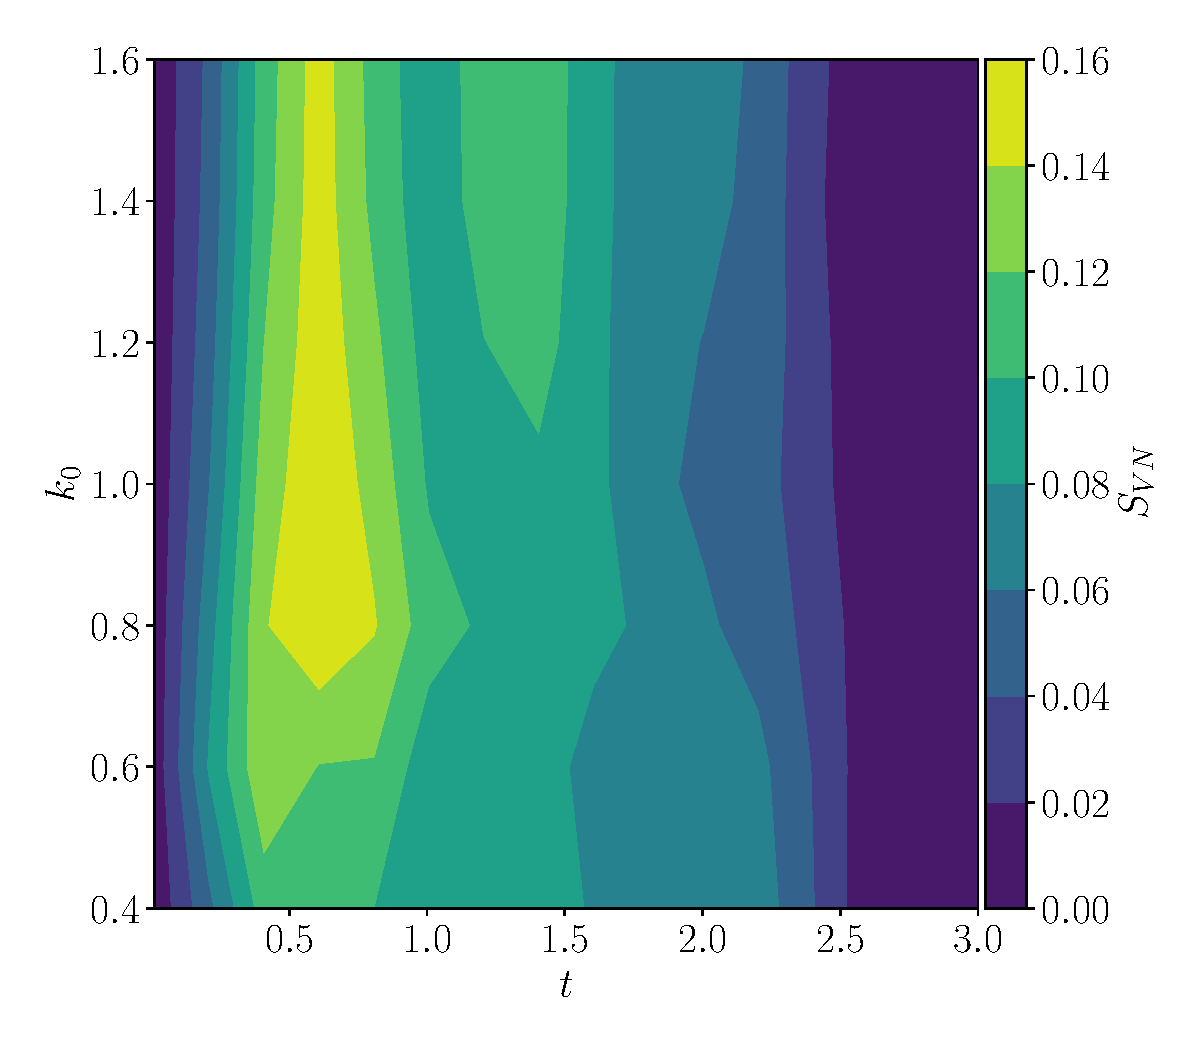
\includegraphics[width=0.46\textwidth]{figures/report_08_2025/entropy_phase_diagram_L_=21_bw=2.0_Jp=1.0_om=0.3.pdf}
    \caption{Phase diagram of the Von Neumann entropy $S_{\rm{VN}}$, for a QPC of size $L=21$ and coupling $\Omega=0.3$.}
    \label{fig:S_phase_diagram}
\end{figure}


\section{Schmidt decomposition}

\begin{align}\label{eq:psi_1}
    \ket{\phi_\nu^{(1)} (k)} = & \frac{1}{(N+1)}\sum_{p\neq k} \ket{p}\otimes \left \{ \frac{ \xi(k,p)}{ -2J( \cos k - \cos p ) } \ket{\nu} + \overbrace{\frac{ \xi(k,p)}{ 2\epsilon_\nu -2J( \cos k - \cos p )} \ket{\mu}}^{\text{Band mixing term}} \right \} \nonumber \\ 
    & + \frac{1}{(N+1)} \frac{\xi(k,k)}{2\epsilon_\nu} \ket{k}\otimes\ket{\mu},
\end{align}

\begin{tcolorbox}[title=QPC eigenstates, colback=white, colframe=black]
\begin{align}
    \bra{n}\ket{k} = \sqrt{\frac{2}{N+1}} \sin(n k) ,\quad & E(k) = -2J\cos(k), \quad k = \frac{n\pi}{N+1},\quad n= 1, 2,...N
\end{align}
Here $\ket{n}$ is the position basis.
\end{tcolorbox}

\begin{tcolorbox}[title=Qubit eigenstates, colback=white, colframe=black]
\begin{align}
   & \ket{+} = \frac{1}{\sqrt{2}}\left( \ket{0} + e^{i\phi} \ket{1}\right), \quad \epsilon_+ = t \\
   & \ket{-} = \frac{1}{\sqrt{2}}\left( \ket{0} - e^{i\phi} \ket{1}\right), \quad \epsilon_- = -t
\end{align}
\end{tcolorbox}

\begin{tcolorbox}[title=Degeneracy Condition, colback=white, colframe=black]
Only $k$-momenta that fulfill
\begin{align}\label{eq:degen_condition}
    & \text{For the symmetric band ($\nu = +$): } -1 \leq \frac{t}{J} + \cos{k} \leq 1 \\
    & \text{For the anti-symmetric band ($\nu = -$): } -1 \leq -\frac{t}{J} + \cos{k} \leq 1
\end{align}
can contribute to the degeneracy, otherwise $\cos p= \pm t/J + \cos k$ has no solution.
\end{tcolorbox}

\begin{tcolorbox}[title=Band-Gap condition, colback=white, colframe=black]
    The perturbative expansion \eqref{eq:psi_1} is well-behaved only when $2\epsilon_\nu \neq \Delta E(k)$. This is always true, when $t/J>1$ and near the middle of the band when
    For momenta near the middle of the band
\begin{align}\label{eq:band_gap_condition}
    \frac{t}{J}<\frac{\pi}{N+1}, \quad \text{ For $k\approx\pi/2$ }.
\end{align}
\end{tcolorbox}

\begin{figure}[h]
    \centering
    \begin{subfigure}[b]{0.43\textwidth}
        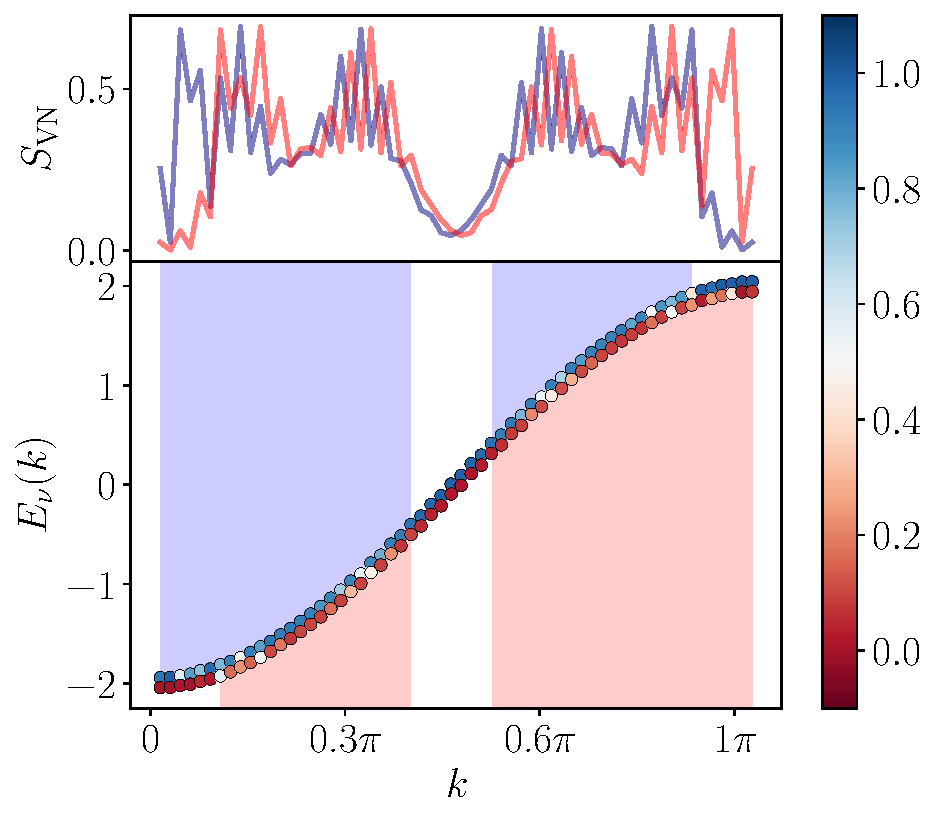
\includegraphics[width=\textwidth]{figures/report_08_2025/exact_energies_Lqpc=60_Omega=0.4_t=0.05.pdf}
        \caption{}
    \end{subfigure}
    \hspace{0.001\textwidth}
    \begin{subfigure}[b]{0.43\textwidth}
        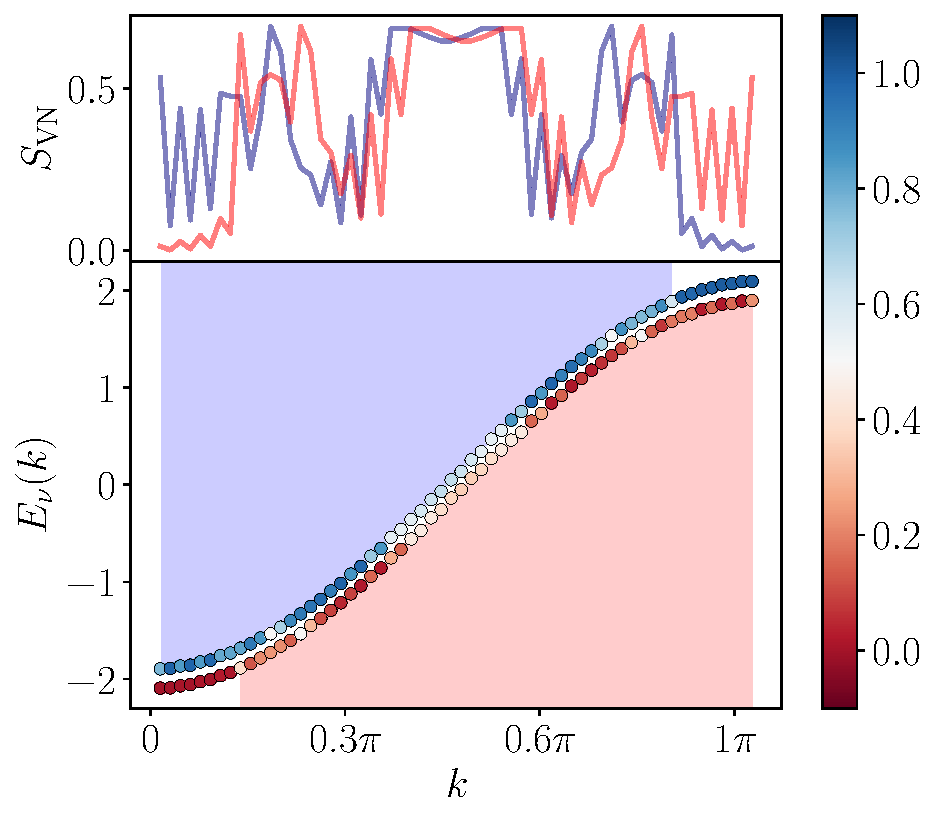
\includegraphics[width=\textwidth]{figures/report_08_2025/exact_energies_Lqpc=60_Omega=0.4_t=0.1.pdf}
        \caption{ }
    \end{subfigure}
    \caption{Exact band structure and entropy contributions of the coupled systems for a QPC of size $L=60$ and $\Omega=0.4$, where (a) depicts the case with Rabi frequency $t=0.05$ and (b) with $t=0.1$. The upper plot shows the entropy that each eigenstate $\ket{\phi_\nu (k)}$ contributes, with the blue line corresponding to the symmetric band and the red line to the antisymmetric one. The lower one shows the eigenenergies sorted into bands, where the color corresponds to the projection of the eigenstate onto the symmetric (blue) and antisymmetric (red) states. The (also color-coded) shaded areas indicate the regions where the perturbative expansion \eqref{eq:psi_1} is degenerate, according to conditions Eq.\eqref{eq:degen_condition} and Eq.\eqref{eq:band_gap_condition}.}
    \label{fig:energy_bands}
\end{figure}


\begin{figure}[h]
    \centering
    \begin{subfigure}[b]{0.43\textwidth}
        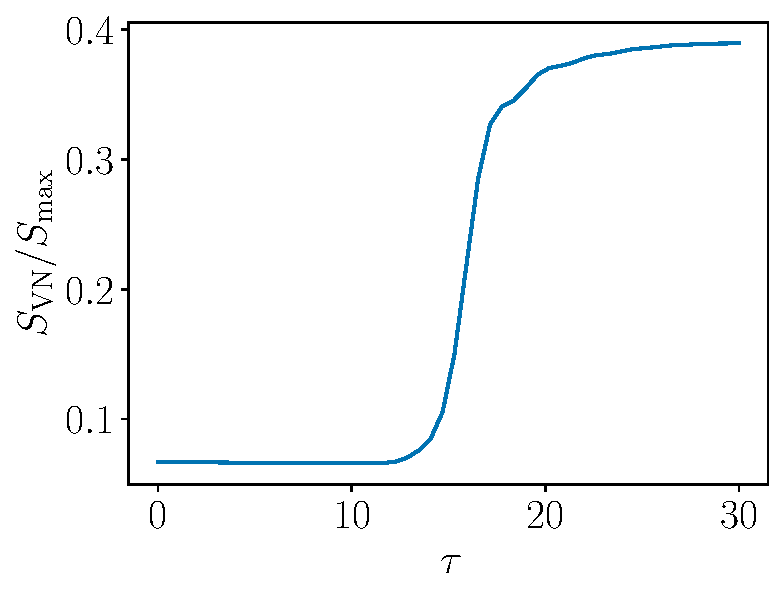
\includegraphics[width=\textwidth]{figures/report_08_2025/entropy_time_exact_Lqpc=60_Omega=0.4_t=0.05.pdf}
        \caption{}
    \end{subfigure}
    \hspace{0.001\textwidth}
    \begin{subfigure}[b]{0.43\textwidth}
        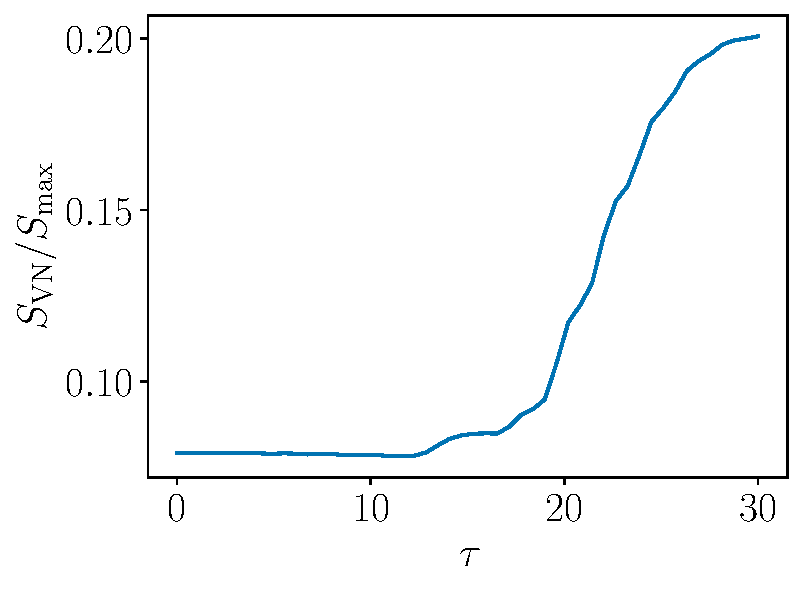
\includegraphics[width=\textwidth]{figures/report_08_2025/entropy_time_exact_Lqpc=60_Omega=0.4_t=0.1.pdf}
        \caption{}
    \end{subfigure}
    \caption{Entanglement entropy a function of time $\tau$ between a QPC Gaussian wave-packet with central momentum $k_0 = \pi/2$ and a qubit. The detector-systems are the same as those shown in figure \ref{fig:energy_bands}, with (a) $t=0.05$ and (b)$t=0.1$. The entropy is normalized by $S_{\rm{max}} = \log(2)$, being the singlet entropy.}
    \label{fig:entropy_in_time}
\end{figure}

\begin{figure}[h]
    \centering
    \begin{subfigure}[b]{0.7\textwidth}
        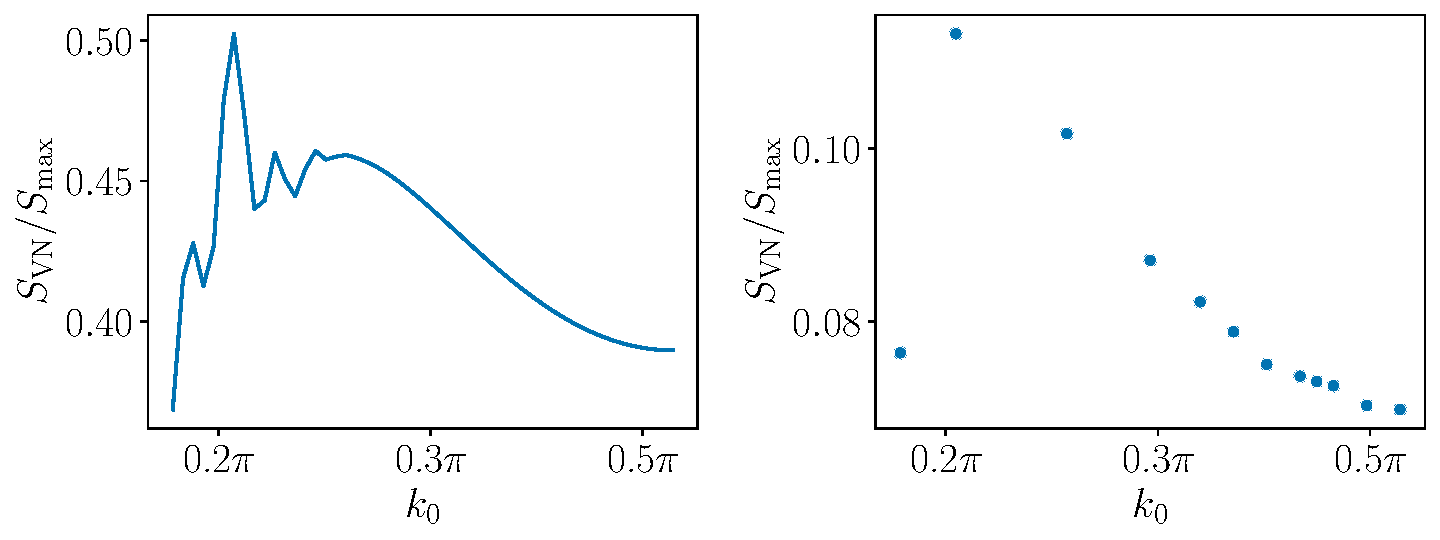
\includegraphics[width=\textwidth]{figures/report_08_2025/wavepacket_entropies_Lqpc=60_Omega=0.4_t=0.05.pdf}
        \caption{}
    \end{subfigure}
    \vspace{0.001\textwidth}
    \begin{subfigure}[b]{0.7\textwidth}
        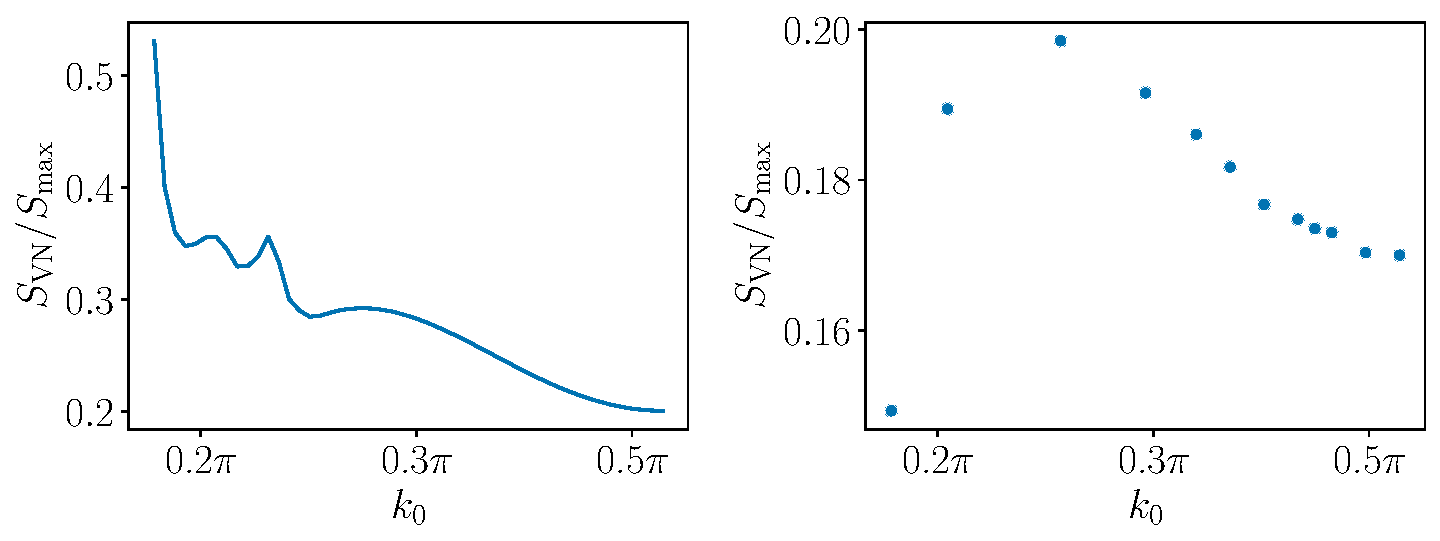
\includegraphics[width=\textwidth]{figures/report_08_2025/wavepacket_entropies_Lqpc=60_Omega=0.4_t=0.1.pdf}
        \caption{}
    \end{subfigure}
    \caption{Final Entropy of a wave packet with the same parameters as in figure \ref{fig:entropy_in_time} and several $k_0$ for (a) $t=0.05$ and (b) $t=0.1$. The solid lines correspond to a QPC with $L=60$ and the points to $L=21$.}
    \label{fig:wave_packet_entropy}
\end{figure}

If we had a free wavepacket, the transmission coefficient will be
\begin{align}\label{eq:transmission_coef}
T = \left( \frac{\Delta^2}{\pi}\right)^{1/2} \int_{-\infty}^{\infty}  \, dk \frac{e^{-(k-k_{0})^2\Delta^2}}{1+\left(\frac{m V_{0}}{k}\right)^2 },
\end{align}
with $V_0 = J \Omega \langle \hat{n}_0(\tau_{\rm{hit}}) \rangle $

\begin{figure}[h]
    \centering
    \begin{subfigure}[b]{0.7\textwidth}
        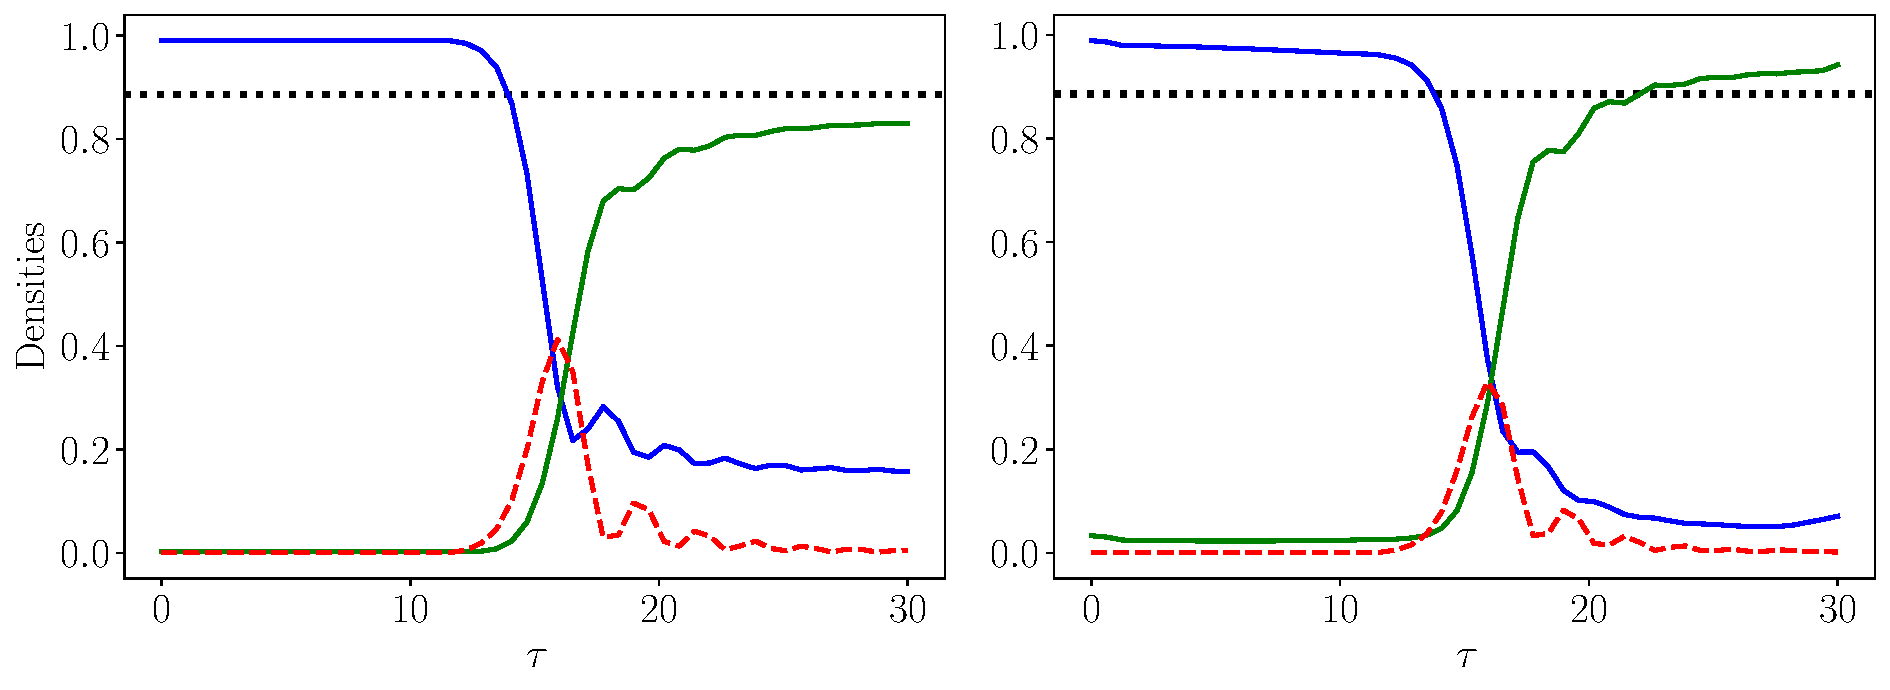
\includegraphics[width=\textwidth]{figures/report_08_2025/occupations_Lqpc=60_Omega=0.4_t=0.05.pdf}
        \caption{}
    \end{subfigure}
    \vspace{0.001\textwidth}
    \begin{subfigure}[b]{0.7\textwidth}
        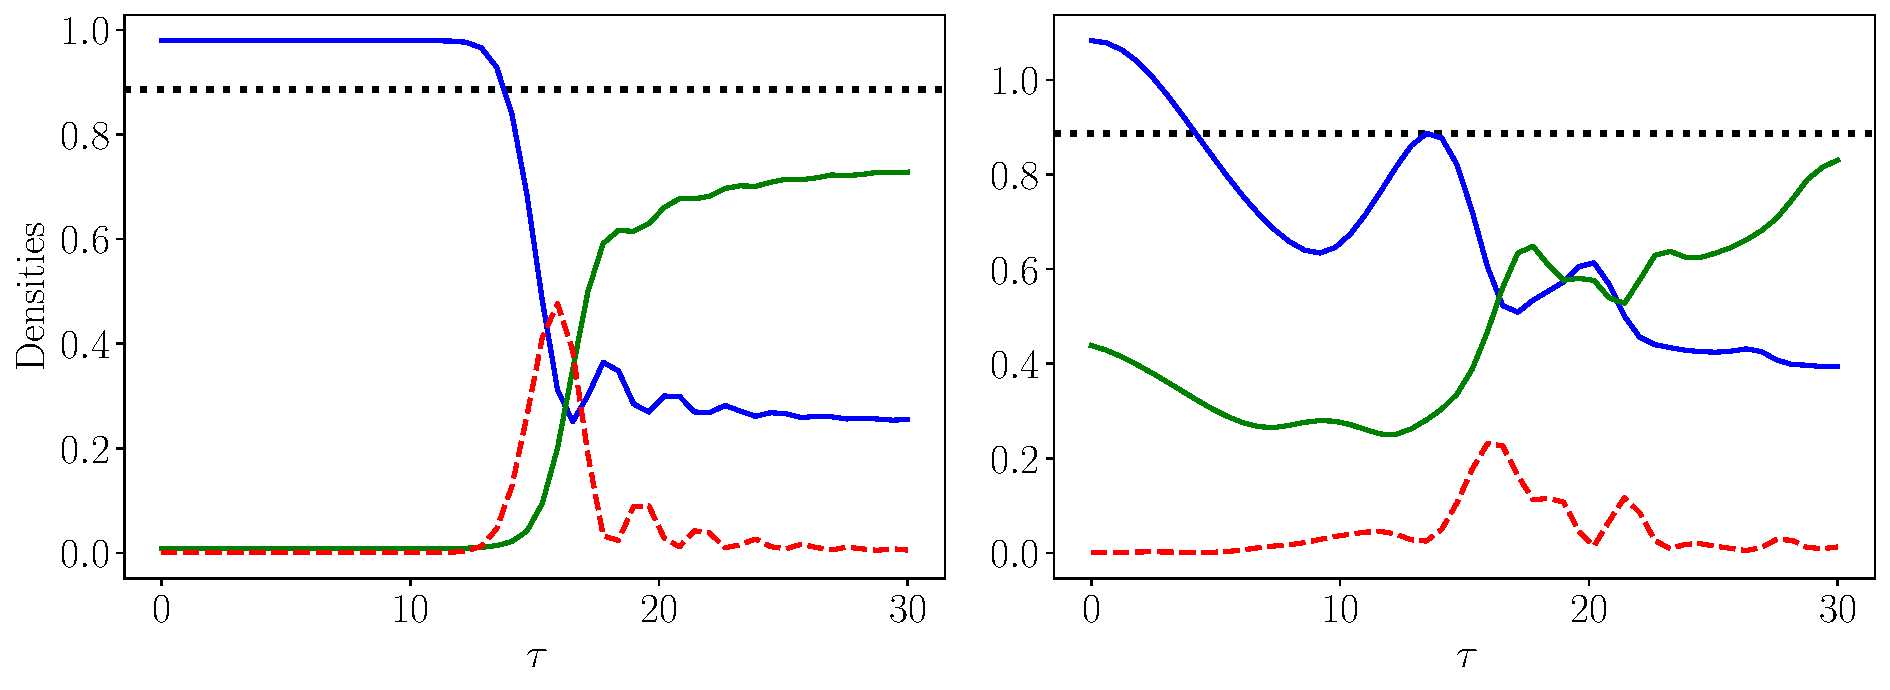
\includegraphics[width=\textwidth]{figures/report_08_2025/occupations_Lqpc=60_Omega=0.4_t=0.1.pdf}
        \caption{}
    \end{subfigure}
    \caption{Occupations for the same system shown in figure \ref{fig:entropy_in_time} where (a) $t=0.05$ and (b) $t=0.1$. The left column depicts the results for the exact eigenstates and the right one, the results with the perturbative eigenstates from Eq.\eqref{eq:psi_1}. The blue solid line, represents the occupations to the left of the bond, the green solid line the occupations to the right of the bond and the red dashed lines the occupations directly at the bond. The black dashed lines are the transmission coefficients from Eq.\eqref{eq:transmission_coef}. }
    \label{fig:occupations}
\end{figure}


\bibliography{qpc}
\bibliographystyle{ieeetr}


\end{document}